\documentclass[10.5pt,fontset=fandol]{ctexart}
\usepackage[paperwidth=222.6413mm,paperheight=297mm,left=1.9cm,right=1.9cm,top=2.1cm,bottom=1.8cm,headsep=0.5cm]{geometry}
\usepackage{amsmath,amssymb,mathrsfs}
\usepackage[table]{xcolor}
\usepackage{booktabs,tabularx,xltabular,needspace,array,ragged2e,enumitem,tcolorbox,tikz,fancyhdr}
\tcbuselibrary{skins,breakable}
\usepackage[hidelinks]{hyperref}
\definecolor{deepblue}{HTML}{1B3A5C}\definecolor{navy}{HTML}{1B3A5C}\definecolor{accentred}{HTML}{B23A48}\definecolor{accentA}{HTML}{B23A48}
\definecolor{muted}{HTML}{5A6470}\definecolor{qbg}{HTML}{F4F6F8}\definecolor{linec}{HTML}{9AA3AD}
\newcolumntype{L}[1]{>{\RaggedRight\arraybackslash}p{#1}}
\newlist{qp}{enumerate}{1}\setlist[qp]{label=(\alph*),leftmargin=1.5em,itemsep=2pt}
\newlist{qn}{enumerate}{1}\setlist[qn]{label=(\arabic*),leftmargin=1.5em,itemsep=2pt}
\newlist{qparts}{enumerate}{1}\setlist[qparts]{label=(\alph*),leftmargin=1.5em,itemsep=2pt}
\newlist{qnum}{enumerate}{1}\setlist[qnum]{label=(\arabic*),leftmargin=1.5em,itemsep=2pt}
\newlist{bul}{itemize}{1}\setlist[bul]{label=\textbullet,leftmargin=1.5em,itemsep=2pt}
\newcommand{\key}[1]{\par\vspace{4pt}\noindent\textbf{\color{navy}#1}\par\vspace{2pt}}
\newcommand{\hint}[1]{\par\smallskip{\small\itshape Hint: #1}\par}
\newcommand{\sect}[1]{{\small\color{muted}#1}}
\newcommand{\dd}{\mathrm d}\newcommand{\Var}{\operatorname{Var}}\newcommand{\Cov}{\operatorname{Cov}}
\newcommand{\E}{\mathbb E}\newcommand{\ee}{\mathrm e}\newcommand{\jj}{\mathrm j}
\newtcolorbox{workspace}{height fill,enhanced,colback=white,colframe=linec!55,boxrule=0.5pt,arc=1.5pt}
\newcommand{\qtitle}[2]{\par\addvspace{1.2em}\Needspace{8\baselineskip}\begin{tcolorbox}[colback=navy,colframe=navy,arc=1.5pt,boxrule=0pt]\color{white}\large\bfseries #1\hfill\small #2\end{tcolorbox}}
\pagestyle{fancy}\fancyhf{}\fancyhead[L]{\footnotesize\color{navy}SSA -- Chapter 2 -- Solutions}\fancyhead[R]{\footnotesize\thepage}
\fancyfoot[C]{\scriptsize Eight-paper edition -- 2026-10-13}
\begin{document}

\begin{titlepage}\centering\vspace*{1.5cm}
{\Huge\bfseries 随机信号分析}\par\vspace{1cm}
{\LARGE\bfseries 第2章复习习题集中文详解}\par\vspace{1cm}
{\large 八套真题版 · 27题 · 9天 · 每天3题}\par\vspace{1cm}
\begin{tcolorbox}[colback=qbg,colframe=navy]
本章八套独占核心均值为15.625分/套；最近四套为9.00分/套。解答按配套英文题集编号，每题保留来源及教材小节。原题条件不足时明确写出可确定的结论与额外假设；奇异高斯分布不强套普通PDF。
\end{tcolorbox}\vfill 2026-10-13\end{titlepage}
\section*{题号与来源索引}
{\small\renewcommand{\arraystretch}{1.15}\begin{xltabular}{\textwidth}{@{}r r L{7cm} X@{}}\toprule 题 & 天 & 题源 & 教材小节\\\midrule\endfirsthead\toprule 题 & 天 & 题源 & 教材小节\\\midrule\endhead\midrule\multicolumn{4}{r}{\small 索引续下页}\\\endfoot\bottomrule\endlastfoot
1 & 1 & Recall / extension & 2.4.1--2.4.3\\
2 & 1 & Textbook 2.19 / Required & 2.4.1\\
3 & 1 & Textbook 2.17 / translated & 2.4.1 / 2.4.3\\
4 & 2 & Adapted from 2022--23 Q3 & 2.4.3\\
5 & 2 & Textbook 2.16 / Required & 2.4.1 / 2.4.3\\
6 & 2 & Textbook 2.18 / Optional & 2.4.1 / 2.4.3\\
7 & 3 & Adapted from 2022--23 Q2(a,b) & 2.2.1 / 2.5\\
8 & 3 & Adapted from 2024--25 Q1 & 2.3.2 / 2.5\\
9 & 3 & Textbook 2.11 / Optional & 2.3.2 / 2.5\\
10 & 4 & Recall / extension & 2.1.3 / 2.3.3\\
11 & 4 & Adapted from 2022--23 Q1 & 2.1.1--2.1.3\\
12 & 4 & Recall / extension & 2.3.1 / 2.5\\
13 & 5 & Textbook 2.3 / Required & 2.1.2 / 2.3.1\\
14 & 5 & Adapted from 2025--26 Q1 & 2.1.2 / 2.3.1 / 2.5\\
15 & 5 & Textbook 2.1 / Optional & 2.1.1 / 2.2.1\\
16 & 6 & Textbook 2.4 / Optional & 2.2.2\\
17 & 6 & Textbook 2.8 / Optional & 2.2.2 / 2.1.3\\
18 & 6 & Textbook 2.7 / Optional & 2.4.2 / 2.1.3\\
19 & 7 & Textbook 2.13 / Required & 2.2.1 / 2.3.4\\
20 & 7 & Textbook 2.14 / translated & 2.3.4\\
21 & 7 & Adapted from 2023--24 Q2(c) & 2.4.3\\
22 & 8 & Adapted from 2018--19 Q3 (201812) & 2.2.1 / 2.4.2 / 2.4.3\\
23 & 8 & 2020--21 / 2021--22 Q1; extended (202104/202112) & 2.4.1 / 2.4.3 / 2.1.3\\
24 & 8 & Adapted from 2019--20 Q3 (201912) & 2.2.3 / 2.1.3\\
25 & 9 & Adapted from 2018--19 Q4 / 2019--20 Q4 & 2.2.1 / 2.5; extension 4.1\\
26 & 9 & Adapted from 2019--20 Q5 (201912) & 2.2.1 / 2.4.3; extension 4.1\\
27 & 9 & 2021--22 Q2(a,b); extensions (202112) & 2.3.2 / 2.5; extension 3.1\\
\end{xltabular}}\par\smallskip 习题与详解题号完全一致；Day标签用于安排，不表示题目在原卷中的顺序。\clearpage
\qtitle{第 1 题}{Day 1}
{\small\color{accentred}(Recall / extension)}\par\smallskip
{\small\color{muted}教材小节：2.4.1--2.4.3}\par\medskip
\noindent\textbf{Gaussian checklist}\par\smallskip\begin{tcolorbox}[breakable,colback=qbg,colframe=qbg,boxrule=0pt]\key{定义与两个不同条件}
由§2.4.3，任意有限个时刻的采样向量都联合高斯，才称为高斯过程。仅每个$X(t)$各自高斯不够。
由§2.4.1，对$C\succeq0$，包括奇异情形，均有
\[\phi_{\boldsymbol X}(u)=\exp(ju^T\mu-\tfrac12u^TCu).\]
普通$n$维PDF还要求$C$正定：
\[f(x)=\frac{e^{-\frac12(x-\mu)^TC^{-1}(x-\mu)}}{(2\pi)^{n/2}\sqrt{\det C}}.\]
若$C$奇异，存在非零$a$使$\Var(a^TX)=a^TCa=0$，于是$a^TX=a^T\mu$几乎必然；分布集中在低维超平面，没有普通$n$维密度。
\key{线性变换}
由§2.4.2，$Y=GX+b$仍联合高斯，$\mu_Y=G\mu+b$，$C_Y=GCG^T$。用特征函数代入$G^Tu$即可证明，无须求可逆变换。
\key{反例与独立判据}
取$Z\sim N(0,1)$，$S$为独立等概正负号，令$X=Z,Y=SZ$。两者边缘都为标准正态，且$E(XY)=E(S)E(Z^2)=0$，但$X^2=Y^2$，故不独立，也不联合高斯。
若\textbf{已经联合高斯}，互不相关才等价于独立：$C$对角时特征函数分解为各边缘特征函数的乘积。这一证明也适用于退化分量。

\end{tcolorbox}
\qtitle{第 2 题}{Day 1}
{\small\color{accentred}(Textbook 2.19 / Required)}\par\smallskip
{\small\color{muted}教材小节：2.4.1}\par\medskip
\noindent\textbf{Joint Gaussian PDF and CF}\par\smallskip\begin{tcolorbox}[breakable,colback=qbg,colframe=qbg,boxrule=0pt]\key{先验算协方差矩阵}
由§2.4.1，$\det C=2\cdot5-3^2=1$，顺序主子式为$2,1$，均为正，因此普通二维密度存在。
\[C^{-1}=\begin{bmatrix}5&-3\\-3&2\end{bmatrix}.\]
令$z_1=x-2,z_2=y-2$。二次型为
\[z^TC^{-1}z=5z_1^2-6z_1z_2+2z_2^2.\]
代入二维高斯密度：
\[\boxed{f_{XY}(x,y)=\frac1{2\pi}\exp\!\left[-\frac{5(x-2)^2-6(x-2)(y-2)+2(y-2)^2}{2}\right].}\]
支持集为整个$\mathbb R^2$，交叉项系数是$-6$，不是$-3$，因为两个非对角元素都贡献一项。
\key{特征函数}
按定义$\phi_{XY}(u,v)=E[e^{j(uX+vY)}]$。利用高斯公式，
\[(u,v)\mu=2u+2v,\qquad (u,v)C(u,v)^T=2u^2+6uv+5v^2.\]
\[\boxed{\phi_{XY}(u,v)=e^{j(2u+2v)-u^2-3uv-\frac52v^2}.}\]
\key{核对}
$\phi(0,0)=1$；$\phi(u,0)=e^{j2u-u^2}$对应$N(2,2)$；$\phi(0,v)=e^{j2v-5v^2/2}$对应$N(2,5)$。交叉协方差为3，因此$X,Y$不独立。

\end{tcolorbox}
\qtitle{第 3 题}{Day 1}
{\small\color{accentred}(Textbook 2.17 / translated)}\par\smallskip
{\small\color{muted}教材小节：2.4.1 / 2.4.3}\par\medskip
\noindent\textbf{Fourth-order Gaussian moment}\par\smallskip\begin{tcolorbox}[breakable,colback=qbg,colframe=qbg,boxrule=0pt]\key{用§2.4.1的高斯特征函数导出矩母函数}
记$C_{ij}=E(X_iX_j)$，零均值联合高斯向量的矩母函数为
\[M(s)=E[e^{s^TX}]=\exp\!\left(\frac12s^TCs\right).\]
高斯矩母函数在原点邻域可微，故$E(X_1X_2X_3X_4)$等于$M(s)$中$s_1s_2s_3s_4$的系数（各变量次数均为1）。
令$Q=\tfrac12s^TCs=\tfrac12\sum_i C_{ii}s_i^2+\sum_{i<j}C_{ij}s_is_j$，展开
\[M(s)=1+Q+\frac{Q^2}{2!}+\cdots.\]
$Q$是二次多项式，只有$Q^2/2$能贡献四次项。四个不同的指标只有三种两两配对：
\[(12)(34),\qquad(13)(24),\qquad(14)(23).\]
每对因子的两种顺序抵消外面的$2!$，所以所求系数为
\[\boxed{C_{12}C_{34}+C_{13}C_{24}+C_{14}C_{23}.}\]
这个推导不依赖$C^{-1}$，所以奇异高斯向量、重合时刻也成立。
\key{考试常用特例}
令$X_1=X_2=X(s)$、$X_3=X_4=X(t)$，得到
\[E[X^2(s)X^2(t)]=E[X^2(s)]E[X^2(t)]+2R_X(s,t)^2.\]
若四个时刻全相同，则$E[X^4(t)]=3\sigma^4(t)$。\textbf{零均值}是上述直接写法的前提；有均值时须先中心化。

\end{tcolorbox}
\qtitle{第 4 题}{Day 2}
{\small\color{accentred}(Adapted from 2022--23 Q3)}\par\smallskip
{\small\color{muted}教材小节：2.4.3}\par\medskip
\noindent\textbf{Gaussian signal through a square-law device}\par\smallskip\begin{tcolorbox}[breakable,colback=qbg,colframe=qbg,boxrule=0pt]\key{(1) 先得到滤波输出的二阶量（第五章工具）}
\[S_X(\omega)=\frac{N_0/2}{1+(\omega RC)^2}.\]
用$e^{-b|\tau|}\leftrightarrow2b/(b^2+\omega^2)$，令$T_c=RC$，得
\[R_X(\tau)=\frac{N_0}{4T_c}e^{-|\tau|/T_c},\qquad v:=\Var X=\frac{N_0}{4T_c}.\]
线性系统保持高斯性，输出零均值。这里$v$表示方差，故其平方为$v^2$。
\key{(2) 平方器需要高斯四阶矩}
由第3题（§2.4.3对应习题2.17），
\[\begin{aligned}m_Y&=aE(X^2)=av,\\
R_Y(\tau)&=a^2E[X^2(t)X^2(t+\tau)]\\
&=a^2[v^2+2R_X(\tau)^2]\\
&=\boxed{a^2v^2(1+2e^{-2|\tau|/T_c})}.\end{aligned}\]
相关函数必须包含非零均值项，因此
\[\boxed{C_Y(\tau)=R_Y(\tau)-m_Y^2=2a^2v^2e^{-2|\tau|/T_c}.}\]
核对：$R_Y(0)=3a^2v^2$，$\Var Y=2a^2v^2$。
\key{(3) 非线性变换不保持高斯}
$a>0$时$Y\ge0$，$a<0$时$Y\le0$，且均不是常数；非退化正态变量的支持为全实轴，所以$Y$不是高斯。$a=0$时为退化高斯常数0。

\end{tcolorbox}
\qtitle{第 5 题}{Day 2}
{\small\color{accentred}(Textbook 2.16 / Required)}\par\smallskip
{\small\color{muted}教材小节：2.4.1 / 2.4.3}\par\medskip
\noindent\textbf{Gaussian sinusoid}\par\smallskip\begin{tcolorbox}[breakable,colback=qbg,colframe=qbg,boxrule=0pt]\key{由§2.4.2先证明联合高斯}
任意多个$X(t_i)$都是独立高斯向量$(A,B)$的线性变换，故联合高斯。$E(AB)=0$，于是
\[m_X(t)=0,\quad C_X(s,t)=\sigma^2[\cos\omega s\cos\omega t+\sin\omega s\sin\omega t]=\sigma^2\cos\omega(s-t).\]
\key{一维密度}
当$\sigma^2>0$，$X(t)\sim N(0,\sigma^2)$：
\[\boxed{f_X(x;t)=\frac1{\sqrt{2\pi}\sigma}e^{-x^2/(2\sigma^2)}.}\]
\key{二维密度：先检查是否退化}
记$\rho=\cos\omega(t_1-t_2)$，则
\[C=\sigma^2\begin{bmatrix}1&\rho\\\rho&1\end{bmatrix},\quad\det C=\sigma^4(1-\rho^2).\]
当$|\rho|<1$，代入§2.4.1的二维密度公式：
\[\boxed{f(x_1,x_2)=\frac{1}{2\pi\sigma^2\sqrt{1-\rho^2}}\exp\!\left[-\frac{x_1^2-2\rho x_1x_2+x_2^2}{2\sigma^2(1-\rho^2)}\right].}\]
当$\omega(t_1-t_2)=k\pi$，有$X(t_2)=(-1)^kX(t_1)=\rho X(t_1)$，分布集中在直线，\textbf{无普通二维PDF}；可用广义表达
\[f(x_1,x_2)=f_X(x_1;t_1)\delta(x_2-\rho x_1).\]
若$\sigma^2=0$，整个过程为0，边缘分布是$\delta(x)$。若$\rho=0$且方差非零，两时刻样本独立；这是\textbf{联合高斯加零协方差}的结论。

\end{tcolorbox}
\qtitle{第 6 题}{Day 2}
{\small\color{accentred}(Textbook 2.18 / Optional)}\par\smallskip
{\small\color{muted}教材小节：2.4.1 / 2.4.3}\par\medskip
\noindent\textbf{Singular three-dimensional Gaussian law}\par\smallskip\begin{tcolorbox}[breakable,colback=qbg,colframe=qbg,boxrule=0pt]\key{列均值与协方差}
设$Z_i=X(t_i)-2$，$c=\cos(0.5)$、$s=\sin(0.5)$。由§2.4.3，
\[\mu=(2,2,2)^T,\quad C=8\begin{bmatrix}1&c&\cos1\\c&1&c\\\cos1&c&1\end{bmatrix}.\]
令$a=(1,c,\cos1)^T$、$b=(0,s,\sin1)^T$，则$C=8(aa^T+bb^T)$。
$a,b$线性无关，所以$\operatorname{rank}C=2$，$\det C=0$。
\key{普通三维密度不存在}
三角恒等式给出$a_1-2ca_2+a_3=0$及$b_1-2cb_2+b_3=0$，从而
\[\Var(Z_1-2cZ_2+Z_3)=0,\quad \boxed{Z_3=2cZ_2-Z_1\quad\text{几乎必然}.}\]
因此全部概率在二维平面上，不能使用含$C^{-1}$的普通三维PDF公式。
\key{仍可写出的完整分布}
特征函数始终成立：$\phi_X(u)=\exp(ju^T\mu-\tfrac12u^TCu)$。
也可先写非退化的$(Z_1,Z_2)$密度，再用冲激表示第三维：
\[\boxed{f_X(x_1,x_2,x_3)=\frac{\exp[-(z_1^2-2cz_1z_2+z_2^2)/(16s^2)]}{16\pi|s|}\,
\delta(z_3-2cz_2+z_1),\quad z_i=x_i-2.}\]
这是\textbf{广义密度}，不是普通三维函数。对$x_3$积分，冲激项积分为1，得到正规的二维高斯密度；再对其余两维积分等于1。题面要求普通PDF时，正确回答应先说明不存在及原因。

\end{tcolorbox}
\qtitle{第 7 题}{Day 3}
{\small\color{accentred}(Adapted from 2022--23 Q2(a,b))}\par\smallskip
{\small\color{muted}教材小节：2.2.1 / 2.5}\par\medskip
\noindent\textbf{Uniform random phase}\par\smallskip\begin{tcolorbox}[breakable,colback=qbg,colframe=qbg,boxrule=0pt]\key{均值：独立性允许分解期望}
由§2.2.1的均匀随机相位平均，
\[E\cos(\omega_0t+\Theta)=\frac1{2\pi}\int_0^{2\pi}\cos(\omega_0t+\theta)d\theta=0.\]
因此$m_\eta(t)=m_\xi E\cos(\omega_0t+\Theta)=0$。不要求$m_\xi=0$。
\key{自相关：同一相位不能分成两个独立相位}
过程$\xi$与$\Theta$独立，所以
\[R_\eta(s,t)=R_\xi(s,t)E[\cos(\omega_0s+\Theta)\cos(\omega_0t+\Theta)].\]
用$\cos a\cos b=\tfrac12\cos(a-b)+\tfrac12\cos(a+b)$：
\[\begin{aligned}E[\cos(\omega_0s+\Theta)\cos(\omega_0t+\Theta)]
&=\tfrac12\cos\omega_0(s-t)\\&\quad+\frac1{4\pi}\int_0^{2\pi}\cos(\omega_0(s+t)+2\theta)d\theta\\
&=\tfrac12\cos\omega_0(s-t).\end{aligned}\]
令$\tau=t-s$，得
\[\boxed{R_\eta(\tau)=\tfrac12R_\xi(\tau)\cos\omega_0\tau.}\]
\key{平稳判断（衔接§3.1.1）}
均值为常数0；相关仅依赖时差；二阶矩有限。因此$\eta$广义平稳，且$C_\eta=R_\eta$。不能仅凭二阶结果宣布严格平稳。

\end{tcolorbox}
\qtitle{第 8 题}{Day 3}
{\small\color{accentred}(Adapted from 2024--25 Q1)}\par\smallskip
{\small\color{muted}教材小节：2.3.2 / 2.5}\par\medskip
\noindent\textbf{Orthogonal but dependent signals}\par\smallskip\begin{tcolorbox}[breakable,colback=qbg,colframe=qbg,boxrule=0pt]\key{先化简离散时间表达式}
整数$n$使$X[n]=\sin\Phi$、$Y[n]=\cos\Phi$。每次试验生成两条常值序列，不是随$n$重新抽相位。
\[m_X=\frac1\pi\int_0^\pi\sin\phi\,d\phi=\frac2\pi,\qquad m_Y=\frac1\pi\int_0^\pi\cos\phi\,d\phi=0.\]
由§2.3.2定义，对任意$m,n$，
\[R_{XY}(m,n)=\frac1\pi\int_0^\pi\sin\phi\cos\phi\,d\phi=0.\]
所以$C_{XY}(m,n)=R_{XY}-m_Xm_Y=0$。两信号\textbf{正交且互不相关}。
\key{不独立：给出概率反证}
令事件$A=\{X>\sqrt3/2\}$、$B=\{|Y|>1/2\}$。两者分别有正概率，但由$X^2+Y^2=1$可知$A\cap B=\varnothing$，故
\[P(A\cap B)=0\ne P(A)P(B).\]
因此两信号不独立。仅写“有共同相位”还不构成一般性的独立性证明或反证；这里用事件严格判断。
\key{联合平稳（第三章概念）}
任意整数平移都不改变任何样本值，故任意联合有限维分布保持不变，实际为联合严格平稳。二阶矩有限，因而也联合广义平稳。
\[R_X(m,n)=R_Y(m,n)=\tfrac12,\quad C_X=\tfrac12-\tfrac4{\pi^2},\quad C_Y=\tfrac12.\]

\end{tcolorbox}
\qtitle{第 9 题}{Day 3}
{\small\color{accentred}(Textbook 2.11 / Optional)}\par\smallskip
{\small\color{muted}教材小节：2.3.2 / 2.5}\par\medskip
\noindent\textbf{Pairwise versus mutual independence}\par\smallskip\begin{tcolorbox}[breakable,colback=qbg,colframe=qbg,boxrule=0pt]\key{原条件下不能唯一确定互相关}
假定所需二阶矩有限，记$\alpha=\omega t_1,\beta=\omega t_2$。由积化和差，
\[R_{XY}=\tfrac12E[A]E[B]\sin(\alpha-\beta)+\tfrac12E[AB\sin(\alpha+\beta+2\Theta)].\]
第一项可用$A,B$独立分解；第二项不能由“两两独立”分解，因为它是三个变量的联合期望。
由$A\perp\Theta,B\perp\Theta$仍可得$m_X=m_Y=0$，所以$C_{XY}=R_{XY}$。
\key{条件不足的具体反例}
取独立于$\Theta$的等概符号$Z=\pm1$，令$A=Z$、$B=Z\operatorname{sgn}(\sin2\Theta)$。
给定任意$\Theta$，$A,B$各自仍是等概符号；又$\operatorname{sgn}(\sin2\Theta)$等概正负，因此$A,B$也独立。三者确实两两独立，但
\[R_{XY}(0,0)=\tfrac12E[AB\sin2\Theta]=\tfrac12E|\sin2\Theta|=\frac1\pi.\]
对比另取$A,B$为相互独立且与$\Theta$独立的等概符号，此时所有两两边缘分布相同，却$R_{XY}=0$。故题设不能唯一给出结果。
\key{若另加相互独立（条件式答案）}
第二项为零，才有$R_{XY}=\tfrac12E[A]E[B]\sin\omega(t_1-t_2)$。
$\omega\ne0$且时间域容许所有时差时，正交及无关等价于$E[A]E[B]=0$；$\omega=0$时此式恒零。
即使相互独立的等概符号振幅给出$R_{XY}\equiv0$，仍有$X^2(t)+Y^2(t)=1$，一般不独立。原条件下正交/无关取决于未知交叉项，统计独立性也不能统一确定。

\end{tcolorbox}
\qtitle{第 10 题}{Day 4}
{\small\color{accentred}(Recall / extension)}\par\smallskip
{\small\color{muted}教材小节：2.1.3 / 2.3.3}\par\medskip
\noindent\textbf{Correlation identities}\par\smallskip\begin{tcolorbox}[breakable,colback=qbg,colframe=qbg,boxrule=0pt]\key{定义（§2.1.3）}
\[m_X(t)=E[X(t)],\quad R_X(s,t)=E[X(s)X(t)],\quad C_X(s,t)=R_X(s,t)-m_X(s)m_X(t).\]
\[R_X(t,t)=E[X^2(t)]=\Var X(t)+m_X(t)^2.\]
只有零均值时，均方值才等于方差。另有$\int f_X(x;t)dx=1$，而$\int xf_X(x;t)dx=m_X(t)$。
\key{半正定与不等式（§2.3.3）}
取样本向量$\boldsymbol X=(X(t_1),\ldots,X(t_n))^T$及实向量$b$，
\[b^TCb=E\left[\left(\sum_i b_i(X(t_i)-m_X(t_i))\right)^2\right]\ge0.\]
这证明了$C$半正定。对中心化变量用Cauchy--Schwarz，
\[|E[(X(s)-m_s)(X(t)-m_t)]|^2\le E[(X(s)-m_s)^2]E[(X(t)-m_t)^2],\]
即所求$|C_X(s,t)|^2\le C_X(s,s)C_X(t,t)$。等号情形允许确定性线性关系，协方差可能奇异。
\key{差信号的自相关（不预设平稳）}
先乘开两个括号再取期望：
\[\boxed{\begin{aligned}R_Y(s,t)={}&R_X(s+a,t+a)-R_X(s+a,t)\\&-R_X(s,t+a)+R_X(s,t).\end{aligned}}\]
若再给WSS，才可化为$R_Y(\tau)=2R_X(\tau)-R_X(\tau-a)-R_X(\tau+a)$。非平稳时不能用这一简式。

\end{tcolorbox}
\qtitle{第 11 题}{Day 4}
{\small\color{accentred}(Adapted from 2022--23 Q1)}\par\smallskip
{\small\color{muted}教材小节：2.1.1--2.1.3}\par\medskip
\noindent\textbf{A random straight line}\par\smallskip\begin{tcolorbox}[breakable,colback=qbg,colframe=qbg,boxrule=0pt]\key{样本函数：固定一次$U$的结果}
可选$U=\pi/4$与$3\pi/4$，得到两条平行直线。
\begin{center}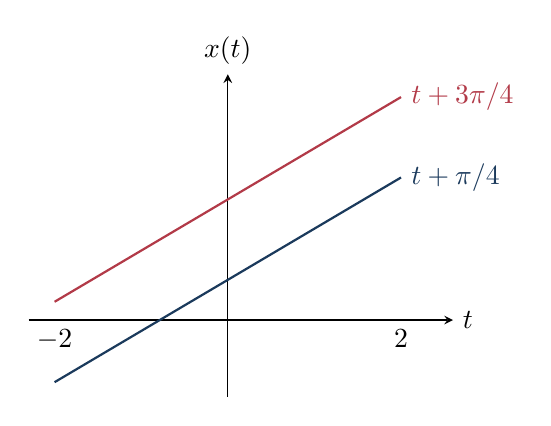
\begin{tikzpicture}[x=1.1cm,y=.65cm,>=stealth]
\draw[->](-2.3,0)--(2.6,0)node[right]{$t$};\draw[->](0,-1.5)--(0,4.8)node[above]{$x(t)$};
\draw[thick,deepblue](-2,-1.215)--(2,2.785)node[right]{$t+\pi/4$};
\draw[thick,accentA](-2,.356)--(2,4.356)node[right]{$t+3\pi/4$};
\node[below]at(-2,0){$-2$};\node[below]at(2,0){$2$};\end{tikzpicture}\end{center}
\key{固定$t$后，对随机变量$U$积分}
\[\phi_{X(t)}(v)=\frac1\pi\int_0^\pi e^{jv(u+t)}du=
\begin{cases}e^{jvt}\dfrac{e^{jv\pi}-1}{jv\pi},&v\ne0,\\1,&v=0.\end{cases}\]
$v$是特征函数的参数，不是过程的随机值；$v=0$处按连续延拓等于1。
\key{数字特征与依赖关系}
\[\boxed{m_X(t)=t+\pi/2,\qquad C_X(s,t)=\Var U=\pi^2/12.}\]
因为$X(t)-m_X(t)=U-\pi/2$对所有时刻相同。
$X(t)-X(s)=t-s$为确定常数，且协方差非零，所以不同时间的样本\textbf{不独立}。均值随$t$变化，也不是WSS。

\end{tcolorbox}
\qtitle{第 12 题}{Day 4}
{\small\color{accentred}(Recall / extension)}\par\smallskip
{\small\color{muted}教材小节：2.3.1 / 2.5}\par\medskip
\noindent\textbf{Independence at the process level}\par\smallskip\begin{tcolorbox}[breakable,colback=qbg,colframe=qbg,boxrule=0pt]\key{过程独立必须覆盖任意多个时刻}
由§2.5，两过程独立指对任意有限时刻$s_1,\ldots,s_m$与$t_1,\ldots,t_n$，向量
$(X(s_1),\ldots,X(s_m))$与$(Y(t_1),\ldots,Y(t_n))$独立，即联合分布分解为两组各自分布的乘积。
对每对单时刻都独立，在一般非高斯情形也未必足以保证上述向量独立；只检查相同时刻更不够。
\key{等时刻独立仍可能跨时刻完全依赖}
题设$X_n=Z_n$、$Y_n=Z_{n-1}$，由于$Z_n,Z_{n-1}$独立，每个固定$n$都有$X_n\perp Y_n$。
但$Y_{n+1}=Z_n=X_n$，因此
\[P(X_n=1,Y_{n+1}=1)=\tfrac12\ne\tfrac12\cdot\tfrac12.\]
两过程不独立。其互相关为
\[R_{XY}(m,n)=E(Z_mZ_{n-1})=\begin{cases}1,&m=n-1,\\0,&m\ne n-1.\end{cases}\]
\key{联合高斯时的充分必要条件}
必须先给出两过程\textbf{联合高斯}。此时两过程独立当且仅当
\[\boxed{C_{XY}(s,t)=0\quad\text{对所有 }s,t.}\]
理由：任意两组采样的联合协方差矩阵交叉块为零，联合高斯特征函数因此按两组分解。非零均值时不能把判据误写成$R_{XY}=0$；应为$R_{XY}(s,t)=m_X(s)m_Y(t)$。

\end{tcolorbox}
\qtitle{第 13 题}{Day 5}
{\small\color{accentred}(Textbook 2.3 / Required)}\par\smallskip
{\small\color{muted}教材小节：2.1.2 / 2.3.1}\par\medskip
\noindent\textbf{One toss, two observation times}\par\smallskip\begin{tcolorbox}[breakable,colback=qbg,colframe=qbg,boxrule=0pt]一次投币决定整条样本函数，所以
\[(X(1/2),X(1))=\begin{cases}(0,-1),&P=1/2,\\(1,2),&P=1/2.\end{cases}\]
由§2.1.2，分布函数取$P(X\le x)$，必须右连续：
\[F_X(x,1/2)=\begin{cases}0,&x<0,\\1/2,&0\le x<1,\\1,&x\ge1,\end{cases}\quad
F_X(x,1)=\begin{cases}0,&x<-1,\\1/2,&-1\le x<2,\\1,&x\ge2.\end{cases}\]
由§2.3.1，联合CDF是同时满足两个门限的原子概率之和：
\[\boxed{F(x_1,x_2)=\tfrac12\mathbf1_{\{x_1\ge0,x_2\ge-1\}}+\tfrac12\mathbf1_{\{x_1\ge1,x_2\ge2\}}.}\]
下图实心端点计入；联合CDF以等高区域表示，各区域高度即函数值。
\begin{center}
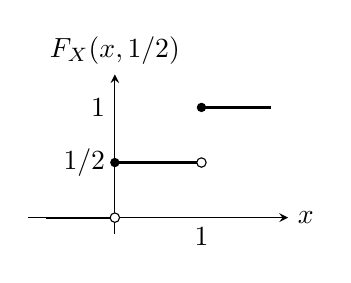
\begin{tikzpicture}[x=1.1cm,y=1.4cm,>=stealth]
\draw[->](-1,0)--(2,0)node[right]{$x$};\draw[->](0,-.15)--(0,1.3)node[above]{$F_X(x,1/2)$};
\draw[thick](-.8,0)--(0,0);\draw[thick](0,.5)--(1,.5);\draw[thick](1,1)--(1.8,1);
\foreach \x/\a/\b in {0/0/.5,1/.5/1}{\draw[fill=white](\x,\a)circle(1.7pt);\fill(\x,\b)circle(1.7pt);}
\node[below]at(1,0){$1$};\node[left]at(0,.5){$1/2$};\node[left]at(0,1){$1$};
\end{tikzpicture}\hspace{13mm}
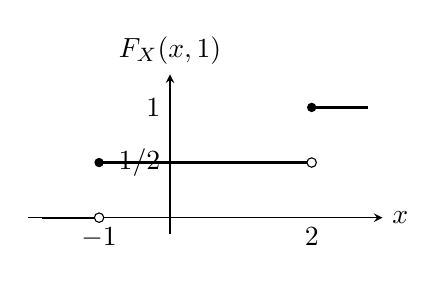
\begin{tikzpicture}[x=.9cm,y=1.4cm,>=stealth]
\draw[->](-2,0)--(3,0)node[right]{$x$};\draw[->](0,-.15)--(0,1.3)node[above]{$F_X(x,1)$};
\draw[thick](-1.8,0)--(-1,0);\draw[thick](-1,.5)--(2,.5);\draw[thick](2,1)--(2.8,1);
\foreach \x/\a/\b in {-1/0/.5,2/.5/1}{\draw[fill=white](\x,\a)circle(1.7pt);\fill(\x,\b)circle(1.7pt);\node[below]at(\x,0){$\x$};}
\node[left]at(0,.5){$1/2$};\node[left]at(0,1){$1$};
\end{tikzpicture}
\end{center}\begin{center}
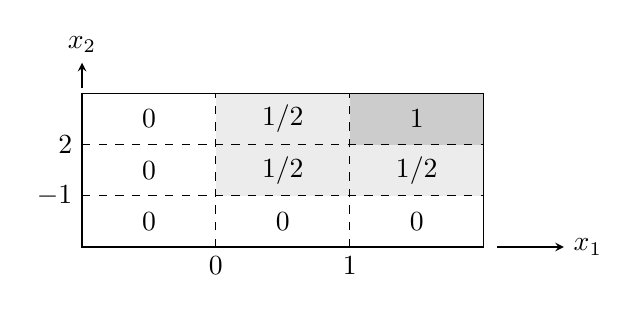
\begin{tikzpicture}[x=1.7cm,y=.65cm,>=stealth]
\fill[gray!15](1,1)rectangle(3,3);\fill[gray!40](2,2)rectangle(3,3);
\draw(0,0)rectangle(3,3);\draw[dashed](1,0)--(1,3);\draw[dashed](2,0)--(2,3);\draw[dashed](0,1)--(3,1);\draw[dashed](0,2)--(3,2);
\foreach \x/\y/\z in {.5/.5/0,1.5/.5/0,2.5/.5/0,.5/1.5/0,1.5/1.5/{1/2},2.5/1.5/{1/2},.5/2.5/0,1.5/2.5/{1/2},2.5/2.5/1}{\node at(\x,\y){$\z$};}
\node[below]at(1,0){$0$};\node[below]at(2,0){$1$};\node[left]at(0,1){$-1$};\node[left]at(0,2){$2$};
\draw[->](3.1,0)--(3.6,0)node[right]{$x_1$};\draw[->](0,3.1)--(0,3.6)node[above]{$x_2$};
\end{tikzpicture}
\end{center}外侧区域向无穷延伸；阈值线属于右侧或上侧区域。联合CDF不是两个边缘CDF的乘积，因为两时刻共享同一次投币。
\end{tcolorbox}
\qtitle{第 14 题}{Day 5}
{\small\color{accentred}(Adapted from 2025--26 Q1)}\par\smallskip
{\small\color{muted}教材小节：2.1.2 / 2.3.1 / 2.5}\par\medskip
\noindent\textbf{One toss versus fresh tosses}\par\smallskip\begin{tcolorbox}[breakable,colback=qbg,colframe=qbg,boxrule=0pt]\key{(1) 一维分布}
$X(2)$取0或4，概率各$1/2$，故
\[\boxed{f_{X(2)}(x)=\tfrac12\delta(x)+\tfrac12\delta(x-4).}\]
这是离散分布的广义密度，不是普通连续密度。
\key{(2) 同次投币：只有两个联合原子}
$(X(1),X(2))$仅可能为$(0,0)$或$(1,4)$，因此
\[\boxed{f(x_1,x_2)=\tfrac12\delta(x_1)\delta(x_2)+\tfrac12\delta(x_1-1)\delta(x_2-4).}\]
\key{(3) 先中心化再相乘}
令$a(t)=\sin2\pi t$，$b(t)=t^2$。均值$m_X(t)=[a(t)+b(t)]/2$。中心化样本为$\pm[a(t)-b(t)]/2$，且所有时刻的正负号相同。因此
\[\boxed{C_X(s,t)=\frac14[\sin(2\pi s)-s^2][\sin(2\pi t)-t^2].}\]
核对$C_X(1,2)=1$，$\Var X(1)=1/4$、$\Var X(2)=4$，相关系数为1。
\key{(4) 每次独立重采样：四个联合原子}
$Y[1]$取0或1，$Y[2]$取0或4，两个选择相互独立：
\[\boxed{f_Y(y_1,y_2)=\tfrac14[\delta(y_1)+\delta(y_1-1)]
[\delta(y_2)+\delta(y_2-4)].}\]
四项概率均为$1/4$。由此可见，单时刻边缘分布相同不意味着过程的联合分布相同。

\end{tcolorbox}
\qtitle{第 15 题}{Day 5}
{\small\color{accentred}(Textbook 2.1 / Optional)}\par\smallskip
{\small\color{muted}教材小节：2.1.1 / 2.2.1}\par\medskip
\noindent\textbf{Random amplitude and a degenerate time}\par\smallskip\begin{tcolorbox}[breakable,colback=qbg,colframe=qbg,boxrule=0pt]\key{(1) 样本函数（题给非负时刻隐含$\omega>0$）}
固定$V=v$得到$x(t)=v\cos\omega t$，例如$v=1/4,3/4$：
\begin{center}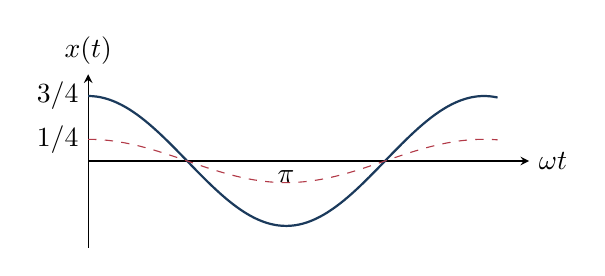
\begin{tikzpicture}[x=.8cm,y=1.1cm,>=stealth]
\draw[->](0,0)--(7,0)node[right]{$\omega t$};\draw[->](0,-1)--(0,1)node[above]{$x(t)$};
\draw[thick,deepblue,domain=0:6.5,samples=100]plot(\x,{.75*cos(\x r)});
\draw[dashed,accentA,domain=0:6.5,samples=100]plot(\x,{.25*cos(\x r)});
\node[left]at(0,.75){$3/4$};\node[left]at(0,.25){$1/4$};\node[below]at(3.14159,0){$\pi$};\end{tikzpicture}\end{center}
\key{(2) 固定时刻的缩放密度}
记$c=\cos\omega t$。$c\ne0$时逆变换$v=x/c$，Jacobian绝对值为$1/|c|$，所以
\[f_X(x;t)=\frac1{|c|}\mathbf1_{\{\min(0,c)\le x\le\max(0,c)\}}.\]
\begin{center}\begin{tabular}{ccc}\toprule 时刻 & $c$ & 非零密度与区间\\\midrule
$0$&1&$1,\quad[0,1]$\\
$\pi/(4\omega)$&$1/\sqrt2$&$\sqrt2,\quad[0,1/\sqrt2]$\\
$3\pi/(4\omega)$&$-1/\sqrt2$&$\sqrt2,\quad[-1/\sqrt2,0]$\\
$\pi/\omega$&$-1$&$1,\quad[-1,0]$\\\bottomrule\end{tabular}\end{center}
负系数会反转区间，但密度不能取负。各区间长度乘密度高度均为1。
\key{(3) 退化时刻}
$t_0=\pi/(2\omega)$使$c=0$，所有样本都等于0，所以$P(X(t_0)=0)=1$。广义密度为$\boxed{\delta(x)}$，不能代入含$1/|c|$的公式。

\end{tcolorbox}
\qtitle{第 16 题}{Day 6}
{\small\color{accentred}(Textbook 2.4 / Optional)}\par\smallskip
{\small\color{muted}教材小节：2.2.2}\par\medskip
\noindent\textbf{Bernoulli words}\par\smallskip\begin{tcolorbox}[breakable,colback=qbg,colframe=qbg,boxrule=0pt]\key{伯努利序列的前提}
由§2.2.2，各比特相互独立且同分布，$p=P(B=1)=0.8$、$q=0.2$。
\key{(1) 指定字串1011}
按顺序相乘：
\[\boxed{P(1011)=pqp^2=p^3q=0.8^3\cdot0.2=0.1024.}\]
这里是指定顺序，不能再乘组合数$\binom43$；后者对应所有“恰好三个1”的字串。
\key{(2) 平均串是均值向量}
以四维向量$\boldsymbol B=(B_1,B_2,B_3,B_4)$表示一个字串，每个$E(B_i)=0.8$，故
\[\boxed{E\boldsymbol B=(0.8,0.8,0.8,0.8).}\]
它不必是某个可实现的二进制串。若把字串解释为二进制整数$W=8B_1+4B_2+2B_3+B_4$，则另有
\[E(W)=(8+4+2+1)\cdot0.8=12.\]
须区分向量的均值与编码后的数值均值。
\key{(3) 最可能的串}
因为$p>q$，把任意0换成1都会使概率乘上$p/q=4$，所以最大概率由全1取得：
\[\boxed{1111,\qquad P(1111)=0.8^4=0.4096.}\]
核对所有16个字串的概率和为$(p+q)^4=1$。

\end{tcolorbox}
\qtitle{第 17 题}{Day 6}
{\small\color{accentred}(Textbook 2.8 / Optional)}\par\smallskip
{\small\color{muted}教材小节：2.2.2 / 2.1.3}\par\medskip
\noindent\textbf{A fair-sign sequence}\par\smallskip\begin{tcolorbox}[breakable,colback=qbg,colframe=qbg,boxrule=0pt]\key{一维分布}
由§2.2.2的伯努利序列含独立性，且每项等概取$-1,+1$，其广义密度为
\[\boxed{f_{I_n}(x)=\tfrac12\delta(x+1)+\tfrac12\delta(x-1).}\]
两个冲激的权重之和为1。不能把离散的概率质量误写成某个区间内的常数密度。
\key{均值与方差}
\[m_I(n)=(-1)\tfrac12+(+1)\tfrac12=0,\quad E(I_n^2)=1,\quad\Var I_n=1.\]
\key{协方差必须分同一指标与不同指标}
由§2.1.3，$C_I(m,n)=E(I_mI_n)-m_I(m)m_I(n)$。若$m\ne n$，独立性给出$E(I_mI_n)=E(I_m)E(I_n)=0$；若$m=n$，$I_n^2=1$。
\[\boxed{C_I(m,n)=R_I(m,n)=\begin{cases}1,&m=n,\\0,&m\ne n.\end{cases}}\]
也可写$\delta_{mn}$（Kronecker delta），但它不是密度中的Dirac冲激$\delta(x)$。
\key{核对独立性的作用}
若只给“每一项边缘等概正负1”，尚不能得到非对角协方差为0，例如所有$I_n$共用同一个符号时，$C_I(m,n)=1$。本题“伯努利序列”使独立性成立。

\end{tcolorbox}
\qtitle{第 18 题}{Day 6}
{\small\color{accentred}(Textbook 2.7 / Optional)}\par\smallskip
{\small\color{muted}教材小节：2.4.2 / 2.1.3}\par\medskip
\noindent\textbf{Gaussian straight-line process}\par\smallskip\begin{tcolorbox}[breakable,colback=qbg,colframe=qbg,boxrule=0pt]\key{确定高斯性}
这里$N(\mu,\sigma^2)$的第二个参数是方差。因为$V,X_0$是独立高斯变量，它们联合高斯。由§2.4.2，固定$t$后的线性组合$X(t)=tV+X_0$仍为高斯。
\key{均值}
期望线性性给出
\[\boxed{m_X(t)=tE(V)+E(X_0)=t.}\]
\key{方差}
先写一般公式再用独立性：
\[\begin{aligned}\Var X(t)&=t^2\Var V+\Var X_0+2t\Cov(V,X_0)\\&=\boxed{t^2+2}.\end{aligned}\]
独立使协方差为0；系数$t$在方差里须平方。
\key{一维密度}
由于$t^2+2>0$始终成立，没有退化时刻：
\[\boxed{f_X(x;t)=\frac1{\sqrt{2\pi(t^2+2)}}\exp\!\left[-\frac{(x-t)^2}{2(t^2+2)}\right],\quad x\in\mathbb R.}\]
换元$z=(x-t)/\sqrt{t^2+2}$可核对积分等于1，而不是等于均值$t$。
\key{延伸核对}
$C_X(s,t)=st+2$，故$C_X(t,t)=t^2+2$与上述一致。均值和方差均随时间变化，过程不广义平稳；这不妨碍其是高斯过程。

\end{tcolorbox}
\qtitle{第 19 题}{Day 7}
{\small\color{accentred}(Textbook 2.13 / Required)}\par\smallskip
{\small\color{muted}教材小节：2.2.1 / 2.3.4}\par\medskip
\noindent\textbf{Random voltage across a parallel RC circuit}\par\smallskip\begin{tcolorbox}[breakable,colback=qbg,colframe=qbg,boxrule=0pt]\key{总电流：沿同一样本函数对时间微分}
按被动符号约定，电阻电流$I_R=X/R$，电容电流$I_C=C\,dX/dt$。每次试验中$A,\Theta$相对于时间固定，因此
\[\frac{dX}{dt}=-A\omega\sin(\omega t+\Theta).\]
总电流为
\[\boxed{I(t)=A\left[R^{-1}\cos(\omega t+\Theta)-\omega C\sin(\omega t+\Theta)\right].}\]
\key{先算幅度和相位的平均}
由均匀密度，$E(A^2)=\tfrac12\int_{-1}^1a^2da=1/3$。
记$\psi=\omega t+\Theta$。均匀相位跨整周期，故
\[E\cos^2\psi=E\sin^2\psi=\tfrac12,\qquad E(\sin\psi\cos\psi)=0.\]
例如$\cos^2\psi=(1+\cos2\psi)/2$，振荡项在完整相位周期上的积分为0。
\key{平方并展开，最后利用独立性}
\[\begin{aligned}E[I^2(t)]&=E[A^2]\{R^{-2}E\cos^2\psi+\omega^2C^2E\sin^2\psi\\&\hspace{33mm}-2\omega CR^{-1}E(\sin\psi\cos\psi)\}\\
&=\boxed{\frac16\left(R^{-2}+\omega^2C^2\right)}.\end{aligned}\]
幅度与相位独立才能这样分解。$E[I]=0$，所以此题均方值也等于方差；一般情况下两者相差均值平方。

\end{tcolorbox}
\qtitle{第 20 题}{Day 7}
{\small\color{accentred}(Textbook 2.14 / translated)}\par\smallskip
{\small\color{muted}教材小节：2.3.4}\par\medskip
\noindent\textbf{Integration of a random signal}\par\smallskip\begin{tcolorbox}[breakable,colback=qbg,colframe=qbg,boxrule=0pt]\key{充分条件}
例如$X(u)$联合可测，且在任意有限区间$[0,T]$满足
$\int_0^T E[X^2(u)]du<\infty$。由Cauchy--Schwarz，这保证均值积分及所需双重积分绝对可积，可用Fubini交换期望与积分，也可按均方积分理解。
\key{均值（§2.3.4）}
\[\boxed{m_Y(t)=E\left[\int_0^tX(u)du\right]=\int_0^t m_X(u)du.}\]
若$m_X$为常数，则$m_Y(t)=tm_X$，积分后的过程一般不平稳。
\key{相关函数：两个上限来自两个时刻}
\[\begin{aligned}R_Y(s,t)&=E\left[\left(\int_0^s X(u)du\right)\left(\int_0^tX(v)dv\right)\right]\\
&=\boxed{\int_0^s\int_0^t R_X(u,v)\,dv\,du}.\end{aligned}\]
同理，
\[C_Y(s,t)=\int_0^s\int_0^t C_X(u,v)\,dv\,du.\]
如果$X$为实值WSS，只能把被积函数化为$R_X(v-u)$，不能因此断言$Y$也WSS。
\key{对角检查}
取$s=t$，$E[Y^2(t)]=\int_0^t\int_0^tR_X(u,v)dvdu$。
若输入WSS，相关函数为偶函数，则
\[E[Y^2(t)]=2\int_0^t(t-\tau)R_X(\tau)d\tau.\]
后一形式用于普通有限二阶矩过程；理想白噪声等广义过程需要分布意义下另行解释。

\end{tcolorbox}
\qtitle{第 21 题}{Day 7}
{\small\color{accentred}(Adapted from 2023--24 Q2(c))}\par\smallskip
{\small\color{muted}教材小节：2.4.3}\par\medskip
\noindent\textbf{White noise is not a Gaussian assumption}\par\smallskip\begin{tcolorbox}[breakable,colback=qbg,colframe=qbg,boxrule=0pt]\key{(1) 只给白噪声，不能推出高斯}
白噪声规定二阶谱为常数，没有规定全部有限维分布。线性系统保持已有高斯性，却不会把任何非高斯输入自动变成精确高斯。因此原条件只能确定$Y$的均值和方差，不能唯一给出其PDF。
例如取高斯白噪声$G$及独立随机幅度$A$，令$P(A=0)=P(A=\sqrt2)=1/2$，$W=AG$。因$E(A^2)=1$，$W$仍具有相同白噪声谱；滤波差分输出却一半概率恒为0，是高斯尺度混合而非非退化高斯。这是按二阶白噪声定义的反例。
\key{(2) 另加高斯假设，才能使用§2.4.3}
滤波和延时差分都是线性操作，故$Y(t)$高斯，且$m_Y=0$。由相关展开，
\[\begin{aligned}v_Y&=E[(X(t)-X(t-T))^2]\\&=2R_X(0)-2R_X(T)\\&=\boxed{\frac{N_0}{2}(1-e^{-T})}>0.\end{aligned}\]
于是
\[\boxed{f_Y(y;t)=\frac1{\sqrt{\pi N_0(1-e^{-T})}}\exp\!\left[-\frac{y^2}{N_0(1-e^{-T})}\right].}\]
注意密度指数的分母是$2v_Y$，归一化系数为$1/\sqrt{2\pi v_Y}$。
\key{(3) $T=0$}
此时$Y(t)\equiv0$，分布是$\delta(y)$，无普通一维密度，不能把$T=0$硬代入上面的非退化公式。

\end{tcolorbox}
\qtitle{第 22 题}{Day 8}
{\small\color{accentred}(Adapted from 2018--19 Q3 (201812))}\par\smallskip
{\small\color{muted}教材小节：2.2.1 / 2.4.2 / 2.4.3}\par\medskip
\noindent\textbf{Gaussian sine and cosine coefficients}\par\smallskip\begin{tcolorbox}[breakable,colback=qbg,colframe=qbg,boxrule=0pt]\key{均值与相关（§2.2.1）}
$E(A)=E(B)=0$给$m_X(t)=0$。独立使$E(AB)=0$，展开乘积得
\[\begin{aligned}R_X(s,t)&=\sigma^2\cos\omega s\cos\omega t+\sigma^2\sin\omega s\sin\omega t\\&=\boxed{\sigma^2\cos\omega(s-t)}.\end{aligned}\]
因此$C_X=R_X$，方差恒为$\sigma^2$。
\key{高斯性与广义平稳}
任何有限个采样值都是联合高斯向量$(A,B)$的线性变换，所以过程高斯（§2.4.2--§2.4.3）。均值恒定、相关只依赖时差，故WSS（§3.1.1）。高斯过程的均值和协方差决定全部有限维分布，故这里也严格平稳。
\key{单独的分量并不WSS}
$W(t)=A\cos\omega t$的方差是$\sigma^2\cos^2\omega t$，$Z(t)=B\sin\omega t$的方差是$\sigma^2\sin^2\omega t$，均随时间变化，因此两者单独都不WSS。原题中的stationary措辞与给定表达式不一致，不能把它当作推导前提。
\key{为何系数方差必须相等}
若分别为$v_A,v_B$，相关含$\tfrac12(v_A-v_B)\cos\omega(s+t)$，仅在相等时这个非平稳项消失。
\end{tcolorbox}
\qtitle{第 23 题}{Day 8}
{\small\color{accentred}(2020--21 / 2021--22 Q1; extended (202104/202112))}\par\smallskip
{\small\color{muted}教材小节：2.4.1 / 2.4.3 / 2.1.3}\par\medskip
\noindent\textbf{Gaussian offset plus cosine}\par\smallskip\begin{tcolorbox}[breakable,colback=qbg,colframe=qbg,boxrule=0pt]\key{单时刻（§2.4.3）}
有限维向量为$(A,B)$的线性变换，故过程高斯。令$c_s=\cos s,c_t=\cos t$。
\[m_X(t)=0,\quad R_X(s,t)=1+c_sc_t,\quad v_t=1+c_t^2>0.\]
\[\boxed{f_X(x;t)=\frac{e^{-x^2/(2v_t)}}{\sqrt{2\pi v_t}}}.\]
\key{协方差与普通二维密度（§2.4.1）}
\[C=\begin{bmatrix}1+c_s^2&1+c_sc_t\\1+c_sc_t&1+c_t^2\end{bmatrix},\quad D=\det C=(c_s-c_t)^2.\]
当$c_s\ne c_t$，$D>0$，普通密度为
\[f(x_1,x_2)=\frac1{2\pi\sqrt D}\exp\!\left[-\frac{(1+c_t^2)x_1^2-2(1+c_sc_t)x_1x_2+(1+c_s^2)x_2^2}{2D}\right].\]
当$c_s=c_t$，两采样值相同，概率集中在$x_2=x_1$；没有普通二维PDF。可用$ f_X(x_1;s)\delta(x_2-x_1)$表达，联合特征函数仍有效。
\key{指定时刻与平稳性扩展}
$(X(0),X(\pi/2))=(A+B,A)$，
\[C=\begin{bmatrix}2&1\\1&1\end{bmatrix},\qquad\phi(u,v)=e^{-[(u+v)^2+u^2]/2}.\]
一般$t$的方差$1+\cos^2t$不恒定，所以不WSS；高斯性不等于平稳性。
\end{tcolorbox}
\qtitle{第 24 题}{Day 8}
{\small\color{accentred}(Adapted from 2019--20 Q3 (201912))}\par\smallskip
{\small\color{muted}教材小节：2.2.3 / 2.1.3}\par\medskip
\noindent\textbf{Semi-random binary transmission}\par\smallskip\begin{tcolorbox}[breakable,colback=qbg,colframe=qbg,boxrule=0pt]\key{均值与同一时隙（§2.2.3）}
$B_k^2=B_k$，故$E(B_k)=E(B_k^2)=1/2$。令$n_1=\lfloor t/T_0\rfloor$，$n_2=\lfloor(t+\tau)/T_0\rfloor$。
\[\boxed{m_X(t)=\tfrac12,\quad R_X(t,t+\tau)=\begin{cases}\tfrac12,&n_1=n_2,\\\tfrac14,&n_1\ne n_2.\end{cases}}\]
不同区间独立才使$E(B_{n_1}B_{n_2})=E(B_{n_1})E(B_{n_2})=1/4$。因此$C_X$同区间为1/4，不同区间为0。
\key{固定边界使相关依赖绝对时刻}
同取$\tau=T_0/2$，$t=0$时两个点同区间，$t=3T_0/4$时跨边界，相关分别1/2与1/4。故不WSS，即使均值和瞬时方差都恒定。
\key{随机滑动后的扩展}
独立均匀时钟滑动使两点落在同一时隙的概率为$p_s=(1-|\tau|/T_0)_+$，其中$(x)_+=\max(x,0)$。按同隙/异隙分解，
\[\boxed{R_Y(\tau)=\tfrac14+\tfrac14(1-|\tau|/T_0)_+},\quad C_Y(\tau)=\tfrac14(1-|\tau|/T_0)_+.\]
$R_Y(0)=1/2$，远时差趋于$1/4=m_Y^2$。原卷是0/1符号，不能直接照搬教材等概正负1的均值0、相关1/0。
\end{tcolorbox}
\qtitle{第 25 题}{Day 9}
{\small\color{accentred}(Adapted from 2018--19 Q4 / 2019--20 Q4)}\par\smallskip
{\small\color{muted}教材小节：2.2.1 / 2.5; extension 4.1}\par\medskip
\noindent\textbf{Random amplitude and uniform phase}\par\smallskip\begin{tcolorbox}[breakable,colback=qbg,colframe=qbg,boxrule=0pt]\key{集合平均（§2.2.1、§2.5）}
由均匀相位，$E_\Theta\cos(\omega t+\Theta)=0$，所以$m_X(t)=0$。利用$2\cos u\cos v=\cos(u-v)+\cos(u+v)$，完整相位周期使和频项平均为0：
\[\boxed{R_X(s,t)=\tfrac12E(A^2)\cos\omega(s-t)}.\]
独立才能把$A^2$和相位项的期望分开。幅度若是任意确定时间函数，不能直接套这个时差形式。
\key{时间平均（第四章扩展）}
固定样本的幅度$a$和相位$\theta$后，正弦积分除以观测长度趋于0，故$\overline X=0$。对乘积用同一三角恒等式，
\[\boxed{\overline R_X(\tau)=\tfrac12A^2\cos\omega\tau}.\]
由于$\omega\ne0$，和频时间平均也为0。
\key{两个各态历经条件不同}
时间均值对每个有限幅度样本等于集合均值0，故均值各态历经。
相关时间平均要几乎必然等于集合相关，令$\tau=0$可知必要条件$A^2=E(A^2)$几乎必然；该条件代入上式也充分。
\[\boxed{\text{相关各态历经}\ \Longleftrightarrow\ A^2\text{几乎必然为常数}}.\]
幅度可有随机正负号，不必$A$本身恒定；随机变化的幅度大小通常使相关不各态历经。
\end{tcolorbox}
\qtitle{第 26 题}{Day 9}
{\small\color{accentred}(Adapted from 2019--20 Q5 (201912))}\par\smallskip
{\small\color{muted}教材小节：2.2.1 / 2.4.3; extension 4.1}\par\medskip
\noindent\textbf{A Gaussian coefficient inside a sign function}\par\smallskip\begin{tcolorbox}[breakable,colback=qbg,colframe=qbg,boxrule=0pt]\key{先看实际进入过程的随机幅度}
记$S=\operatorname{sgn}(A)$。连续正态给$P(A=0)=0$，$S=\pm1$等概，且$S^2=1$几乎必然。
由相位均匀与独立，
\[\boxed{m_X=0,\quad R_X(s,t)=\tfrac12\cos\omega_0(s-t)}.\]
$A$是高斯，不代表非线性函数$S$高斯。
\key{边缘是反正弦分布}
乘以$-1$相当于给均匀相位加$\pi$，所以$X(t)$的边缘与$\cos U$相同，$U\sim U(0,2\pi)$。对$-1<x<1$有两个逆分支，每个$|dx/dU|=\sqrt{1-x^2}$，故
\[\boxed{f_X(x;t)=\frac1{\pi\sqrt{1-x^2}},\quad -1<x<1},\]
区间外为0。这是有界非退化变量，因此不是正态，也不是高斯过程。密度端点可积，$\int_{-1}^1dx/(\pi\sqrt{1-x^2})=1$。
\key{广义各态历经扩展}
每个样本的幅度平方恒为1，时间均值0，时间自相关$\tfrac12\cos\omega_0\tau$，恰好等于集合量。所以均值与相关各态历经都成立。这一例同时说明WSS、各态历经与高斯是不同概念。
\end{tcolorbox}
\qtitle{第 27 题}{Day 9}
{\small\color{accentred}(2021--22 Q2(a,b); extensions (202112))}\par\smallskip
{\small\color{muted}教材小节：2.3.2 / 2.5; extension 3.1}\par\medskip
\noindent\textbf{Delayed radar echo plus independent noise}\par\smallskip\begin{tcolorbox}[breakable,colback=qbg,colframe=qbg,boxrule=0pt]\key{和信号的二阶量（§2.3.2、§2.5）}
期望线性性给$m_Y=0$。展开$Y(t)Y(t+\tau)$，两个交叉项因独立与零均值为0：
\[\boxed{R_Y(\tau)=\alpha^2R_X(\tau)+R_N(\tau)}.\]
同一支路的两时刻都减$d$，因此它的自相关时差仍为$\tau$，不是$\tau-d$。
\key{互相关要固定约定}
\[\begin{aligned}R_{XY}(\tau)&=E[X(t)(\alpha X(t+\tau-d)+N(t+\tau))]\\&=\boxed{\alpha R_X(\tau-d)},\\
R_{YX}(\tau)&=E[(\alpha X(t-d)+N(t))X(t+\tau)]\\&=\boxed{\alpha R_X(\tau+d)}.\end{aligned}\]
实值WSS的$R_X$是偶函数，故$R_{YX}(\tau)=R_{XY}(-\tau)$。前后次序交换会改变时延符号；自相关和互相关不可混用。
\key{平稳性与高斯性分别判断}
$Y$均值恒定、自相关只依赖时差，故WSS；两过程各自WSS且两个互相关只依赖时差，故联合WSS（§3.1）。
这些条件仅规定二阶结构，不推出Gaussian。若另加$X,N$为独立高斯过程，则采样向量的线性组合仍联合高斯，才可断言$Y$高斯。
\end{tcolorbox}
\end{document}